%  LaTeX support: latex@mdpi.com 
%  In case you need support, please attach all files that are necessary for compiling as well as the log file, and specify the details of your LaTeX setup (which operating system and LaTeX version / tools you are using).

% You need to save the "mdpi.cls" and "mdpi.bst" files into the same folder as this template file.

%=================================================================
\documentclass[arts,article,submit,moreauthors,pdftex,10pt,a4paper]{mdpi} 
%
%--------------------
% Class Options:
%--------------------
% journal
%----------
% Choose between the following MDPI journals:
% actuators, addictions, admsci, aerospace, agriculture, agronomy, algorithms, animals, antibiotics, antibodies, antioxidants, applsci, arts, atmosphere, atoms, axioms, batteries, bdcc, behavsci, beverages, bioengineering, biology, biomedicines, biomimetics, biomolecules, biosensors, brainsci, buildings, carbon, cancers, catalysts, cells, challenges, chemengineering, chemosensors, children, chromatography, climate, coatings, colloids, computation, computers, condensedmatter, cosmetics, cryptography, crystals, cybersecurity, data, dentistry, designs, diagnostics, diseases, diversity, econometrics, economies, education, electrochemistry, electronics, energies, entropy, environments, epigenomes, fermentation, fibers, fishes, fluids, foods, forests, fractalfract, futureinternet, galaxies, games, gastrointestdisord, gels, genealogy, genes, geosciences, geriatrics, healthcare, highthroughput, horticulturae, humanities, hydrology, informatics, information, infrastructures, inorganics, insects, instruments, ijerph, ijfs, ijms, ijgi, ijtpp, inventions, jcdd, jcm, jcs, jdb, jfb, jfmk, jimaging, jof, jintelligence, jlpea, jmmp, jmse, jpm, jrfm, jsan, land, languages, laws, life, literature, logistics, lubricants, machines, magnetochemistry, make, marinedrugs, materials, mathematics, mca, mti, medsci, medicines, membranes, metabolites, metals, microarrays, micromachines, microorganisms, minerals, molbank, molecules, mps, nanomaterials, ncrna, neonatalscreening, nitrogen, nutrients, ohbm, particles, pathogens, pharmaceuticals, pharmaceutics, pharmacy, philosophies, photonics, plants, plasma, polymers, proceedings, processes, proteomes, publications, quaternary, qubs, recycling, religions, remotesensing, resources, risks, robotics, safety, scipharm, sensors, separations, sexes, sinusitis, socsci, societies, soils, sports, standards, surgeries, sustainability, symmetry, systems, technologies, toxics, toxins, tropicalmed, universe, urbansci, vaccines, vetsci, viruses, vision, water, wem
%---------
% article
%---------
% The default type of manuscript is article, but can be replaced by: 
% addendum, article, benchmark, book, bookreview, briefreport, casereport, changes, comment, commentary, communication, conceptpaper, correction, conferenceproceedings, conferencereport, expressionofconcern, meetingreport, creative, datadescriptor, discussion, editorial, essay, erratum, hypothesis, interestingimages, letter, newbookreceived, opinion, obituary, projectreport, reply, reprint, retraction, review, perspective, preprints, protocol, shortnote, supfile, technicalnote, viewpoint
% supfile = supplementary materials
% protocol: If you are preparing a "Protocol" paper, please refer to http://www.mdpi.com/journal/mps/instructions for details on its expected structure and content.
%----------
% submit
%----------
% The class option "submit" will be changed to "accept" by the Editorial Office when the paper is accepted. This will only make changes to the frontpage (e.g. the logo of the journal will get visible), the headings, and the copyright information. Also, line numbering will be removed. Journal info and pagination for accepted papers will also be assigned by the Editorial Office.
%------------------
% moreauthors
%------------------
% If there is only one author the class option oneauthor should be used. Otherwise use the class option moreauthors.
%---------
% pdftex
%---------
% The option pdftex is for use with pdfLaTeX. If eps figure are used, remove the option pdftex and use LaTeX and dvi2pdf.

%=================================================================
\firstpage{1} 
\makeatletter 
\setcounter{page}{\@firstpage} 
\makeatother 
\articlenumber{x}
\doinum{10.3390/------}
\pubvolume{xx}
\pubyear{2017}
\copyrightyear{2017}
\externaleditor{Academic Editor: Frederic Fol Leymarie}
\history{Received: date; Accepted: date; Published: date}

%------------------------------------------------------------------
% The following line should be uncommented if the LaTeX file is uploaded to arXiv.org
%\pdfoutput=1

%=================================================================
% Add packages and commands here. The following packages are loaded in our class file: fontenc, calc, indentfirst, fancyhdr, graphicx, lastpage, ifthen, lineno, float, amsmath, setspace, enumitem, mathpazo, booktabs, titlesec, etoolbox, amsthm, hyphenat, natbib, hyperref, footmisc, geometry, caption, url, mdframed, tabto, soul, multirow, microtype, tikz

%=================================================================
%% Please use the following mathematics environments: Theorem, Lemma, Corollary, Proposition, Characterization, Property, Problem, Example, ExamplesandDefinitions, Hypothesis, Remark, Definition
%% For proofs, please use the proof environment (the amsthm package is loaded by the MDPI class).

%=================================================================
% Full title of the paper (Capitalized)
%\Title{Choreographer in Residence at the Robotics, Automation, and Dance (RAD) Lab}
\Title{Choreographic and Somatic Practices Toward the Development of Expressive Robotic Systems}

% If this is an expanded version of a conference paper, please cite it here: enter the full citation of your conference paper, and add $^\dagger$ in the end of the title of this article.
%\conference{Title}

% Author Orchid ID: enter ID or remove command
\newcommand{\orcidauthorA}{0000-0002-9722-9893} % Add \orcidA{} behind the author's name
%\newcommand{\orcidauthorB}{0000-0000-000-000X} % Add \orcidB{} behind the author's name

% Authors, for the paper (add full first names)
\Author{Amy LaViers $^{1}$\orcidA{}*, Catie Cuan$^{2,\dagger}$, Madison Heimerdinger$^{1,\dagger}$, Umer, Huzaifa$^{1,\dagger}$, Catherine Maguire$^{2,3,\dagger}$, Alexandra Niles$^{5,\dagger}$, Karen Bradley$^{2,3,\ddagger}$, Kim Brooks Mata$^{1,\ddagger}$, and Alexander Zurawski$^{1,\ddagger}$} %Ishaan Pakrasi , Novoneel Chakraborty, Reika McNish, Riley Watts, 

% Authors, for metadata in PDF
\AuthorNames{Amy LaViers, Karen Bradley, Kim Brooks Mata, Catie Cuan, Madison Heimerdinger, Umer, Huzaifa, Catherine Maguire, Alexandra Niles, and Alexander Zurawski}  % Novoneel Chakraborty, Ishaan Pakrasi, Reika McNish, Riley Watts, 

% Affiliations / Addresses (Add [1] after \address if there is only one affiliation.)
\address{%
$^{1}$ \quad Mechanical Science and Engineering Department, University of Illinois at Urbana-Champaign\\
$^{2}$ \quad Independent dance artist or professional\\
$^{3}$ \quad Laban/Bartenieff Institute for Movement Studies\\
$^{4}$ \quad Dance Program, University of Virginia\\
$^{5}$ \quad Computer Science Department, University of Illinois at Urbana-Champaign}

% Contact information of the corresponding author
\corres{Correspondence: alaviers@illinois.edu; Tel.: +1-217-300-1486}

% Current address and/or shared authorship
\firstnote{These authors contributed equally to this work.} 
\secondnote{These authors contributed equally to this work.}
% The commands \thirdnote{} till \eighthnote{} are available for further notes

% Simple summary
%\simplesumm{}

% Abstract (Do not use inserted blank lines, i.e. \\) %%%%%%%about 200 words maximum
\abstract{ %As robotic systems move out of factory work cells into human-facing environments questions of choreography become central to their design, placement, and application.  With a human viewer or counterpart present, a system will automatically, necessarily be interpreted within context, style of movement, and form factor by a human being as an animate element of their environment.  The interpretation by this human viewer or interactant is critical to the success of the system’s integration.  Thus, professional choreographers, dance practicitioners, and movement analysts are critical to research in robotics.  This article reports in detail on practices employed by one research lab and specific impacts on technical projects within.
As robotic systems move out of factory work cells into human-facing environments questions of choreography become central to their design, placement, and application.  With a human viewer or counterpart present, a system will automatically, necessarily be interpreted within context, style of movement, and form factor by a human being as an animate element of their environment.  The interpretation by this human counterpart is critical to the success of the system’s integration: ``knobs’’ on the system need to make sense to a human counterpart; an artificial agent should have a way of notifying a human counterpart of a change in system state, possibly through motion profiles; and the motion of a human counterpart may have important contextual clues for task completion.  Thus, professional choreographers, dance practitioners, and movement analysts are critical to research in robotics.  They have design methods for movement that align with human audience perception; they can help identify simplified features of movement that will effectively accomplish human-robot interaction goals; and they have detailed knowledge of the capacity of human movement.  This article details practices employed by one research lab and specific impacts on technical and artistic projects within.
%1) Background: Place the question addressed in a broad context and highlight the purpose of the study; 2) Methods: Describe briefly the main methods or treatments applied; 3) Results: Summarize the article's main findings; and 4) Conclusion: Indicate the main conclusions or interpretations. The abstract should be an objective representation of the article, it must not contain results which are not presented and substantiated in the main text and should not exaggerate the main conclusions.
}

% Keywords
\keyword{robotics; choreography; Laban/Bartenieff Movement System; interdisciplinary collaboration} %(list three to ten pertinent keywords specific to the article, yet reasonably common within the subject discipline.)}

% The fields PACS, MSC, and JEL may be left empty or commented out if not applicable
%\PACS{J0101}
%\MSC{}
%\JEL{}

%%%%%%%%%%%%%%%%%%%%%%%%%%%%%%%%%%%%%%%%%%
% Only for journal Applied Sciences:
%\featuredapplication{Authors are encouraged to provide a concise description of the specific application or a potential application of the work. This section is not mandatory.}
%%%%%%%%%%%%%%%%%%%%%%%%%%%%%%%%%%%%%%%%%%


%%%%%%%%%%%%%%%%%%%%%%%%%%%%%%%%%%%%%%%%%%
% Only for the journal Data:
%\dataset{DOI number or link to the deposited data set in cases where the data set is published or set to be published separately. If the data set is submitted and will be published as a supplement to this paper in the journal Data, this field will be filled by the editors of the journal. In this case, please make sure to submit the data set as a supplement when entering your manuscript into our manuscript editorial system.}

%\datasetlicense{license under which the data set is made available (CC0, CC-BY, CC-BY-SA, CC-BY-NC, etc.)}

%%%%%%%%%%%%%%%%%%%%%%%%%%%%%%%%%%%%%%%%%%
% For Conference Proceedings Papers:
%\conferencetitle{Add the conference title here}

%\setcounter{secnumdepth}{4}
%%%%%%%%%%%%%%%%%%%%%%%%%%%%%%%%%%%%%%%%%%

\usepackage{wrapfig}

\begin{document}
%%%%%%%%%%%%%%%%%%%%%%%%%%%%%%%%%%%%%%%%%%
%% Only for the journal Gels: Please place the Experimental Section after the Conclusions

%%%%%%%%%%%%%%%%%%%%%%%%%%%%%%%%%%%%%%%%%%

\section{Introduction}

\textcolor{red}{just collecting *possibly* useful fragments; I'll write this section at the end}

where the teacher's feedback pointed to the connection between a barr\'{e} exercise (grand battment) and a so-called floor exercise (tour jet\'{e}); this realization led to several publications \cite{laviers2011ACC,laviers2011ICCPS,laviers2011IEEERAM}.  

utilizing the Laban/Bartenieff Movement System (LBMS) to help identify patterns, find embodiment and link the endeavor of human movement to that of robots and their designers.  

The LBMS system and the framework of movement it illuminates is in itself a juncture of art and science, and by extension the rapidly developing world of technology we now live in. Art has always been a means of finding understanding and expressive communication. My work with Amy is about using movement and embodied expression to inform the design of robots that can then be communicative and expressive in their work contexts. 

\begin{itemize}
\item problems publishing with Cat
\item problems funding Catie
\item value experienced over nearly a decade in this work
\end{itemize}

 
%%%%%%%%%%%%%%%%%%%%%%%%%%%%%%%%%%%%%%%%%%
%\section{Background: Two Contributing, Complementary Disciplines}

\subsection{Pervasive Previous Perspectives}

\textcolor{red}{Amy and Karen and Ilya and Cat}

\begin{flushleft}
\textit{\textbf{Domin}: So young Rossum said to himself: Man is a being that does things such as feeling happiness, plays the violin, likes to go for a walk, and all sorts of other things which are simply not needed.\\
\textbf{Domin}: No, wait.  Which are simply not needed for activities such as weaving or calculating.  A petrol engine doesn't have any ornaments or tassels on it, and making an artificial worker is just like making a petrol engine.  The simpler you make production the better you make the product.  What sort of worker do you think is the best?\\
\textbf{Helena}: The best sort of worker?  I suppose one who is honest and dedicated.\\
\textbf{Domin}: No.  The best sort of worker is the cheapest worker.  The one that has the least needs.  What young Rossum invented was a worker with the least needs possible.  He had to make him simpler.  He threw out everything that wasn't of direct use in his work, that's to say, he threw out the man and put in the robot.  Miss Glory, robots are not people.  They are mechanically much better than we are, they have an amazing ability to understand things, but they don't have a soul.  Young Rossum created something much more sophisticated than Nature ever did -- technically at least!}
\end{flushleft}
\vspace{-.2in}
\begin{flushright}
-- RUR (Rossums’ Universal Robots) \cite{vcapek2004rur}
\end{flushright}

Bringing together choreography and engineering raises a question about whether both fields are concerned with the same values and questions. That is, are they motivated by the same organizing principles and can their practices be complementary, and further mutually beneficial, when brought together? 
In this excerpt from the play where the term ``robot'' was coined, the immediate intertwining of robotics and the arts can be observed.  Notice that from the first moment the concept of a ``robot'' was conceived there was an idea injected that movement could be divided between its efficient, functional parts and its extraneous, expressive parts.  Thus, this idea, of efficiency, and function, has permeated robotics since the word was introduced in a 1920 play \cite{vcapek2004rur}.  Long before they were called robots, automatic mechanical machines, automata, have existed since antiquity and as Truitt writes ``are mimetic objects that dramatize the structure of the cosmos and humankind's role in it'' \cite{truitt2015medieval}.

At the same time, a choreographer Rudolf Laban (1879-1958) \cite{bradley2008rudolf} was working to establish a system for movement, now called the Laban/Bartenieff Movement System (LBMS), that helped codify learning from work in the arts and helped frame a rejection of industrialization and return to nature.  Thus, both the \textit{idea} of a robot and the somatic (or ``body-based'') movement system leveraged heavily in the methods presented here are in part a reaction to the industrial revolution where mechanical efficiency was taken to hyperbolic levels not previously seen.  
Dancers’ technique and training often reflects the ethos of developing efficiency through replication of motor tasks, continually refined and streamlined. \textcolor{red}{But dance performance requires the use of something more, maybe the same thing Domin and Helena discuss as missing from the concept of a robot. \textit{the order of this sentence should be reversed}.} 

Thus, as much as physical phenomenon, the distinction between human and robot movement is a philosophical distinction.
In broad, reductive strokes, we argue that both engineers and choreographers aim to do the same thing:  to understand and convey subtleties of movement. One of the fundamental emergent questions from this categorization is the lens through which constituents in each field methodologically approach how to generate, interpret, and reproduce different movement from the idiosyncratic to the robotic.  %To begin to analyze this space, I move to 
Consider two branches of philosophical inquiry, one concerned with \textit{phenomena} and the other with \textit{rhetoric} as a model for understanding the potential differences in assumptions generated from each field. 

Philosophy, broadly speaking, often refers to a rigorous investigation of what it means to lead a good life. The different branches of philosophical inquiry provide critical, albeit artificial, lenses by which to address this complex question. Two such branches, rhetoric and phenomenology, are useful in understanding subjective and intersubjective experience, though notably from different angles. Rhetoric, at least in the classical (Aristotelian) sense, investigates ``the available means of persuasion'' in any given situation \cite{kennedy2006rhetoric}. Outside of ancient Greek life, contemporary rhetoric can be understood as a practice to examine the function, efficiency, and efficacy of persuasive communication—starting with linguistic, and moving to the visual, bodily, energetic, posthuman, and so on \cite{barnett2016rhetoric}. Alternatively, phenomenology provides a lens through which to understand subjective, first-person experience. Championed by Edmund Husserl at the turn of the twentieth century, phenomenology urges a ``bracketing'' of experience such that an individual approaches stimuli as if for the first time \cite{husserl2012ideas}. Phenomenology and rhetoric are not, strictly speaking, incongruous. One can approach the creation of rhetorical artifacts (i.e. speeches, visualizations, choreographies, etc.) phenomenologically, just as one can probe first-person experience rhetorically. It is important to state again that these fields are artificial constructs -- they offer a way by which to view the world but their limitations are neither absolute nor universal.   \textcolor{red}{\textit{I like it, but I think this paragraph might be completely unintelligible to technical audiences.}}

Returning to the questions of engineers and choreographers, a major problem can occur when one falls to deep into the rabbit hole of philosophical inquiry. For engineers, the problem occurs when valuing efficiency and function trump user experience (i.e. phenomenology). For choreographers, the problem occurs when first-person experience (of the performers) is not convincing. As with any practice, balance is imperative. To be able to address complex questions pertaining to generating, interpreting, and reproducing movement, relying too heavily on rhetoric or phenomenology can be limiting in a way that be invisible or simply not salient for the agents. This is one reason, among many, to support bringing engineers and choreographers together into one shared space, and, for a robotics lab, to employ phenomenologically motivated practice in our research. In bridging the first-person experience with questions of efficacy and efficiency, we can move closer to producing truly complex systems. 

In the largest sense, the purpose of the methods presented here is to explore what human bodies can express in movement, what ideas machines can express in movement and whether they are the same things. Can the robot expressively communicate? The other big idea is to utilize the choreography of the body itself and its expressive capabilities to ``move''  engineers into an embodied experience that could inform their work both in design and context creation. Meaning making through movement -- engineering through body.

Thus, here, we take a more pragmatic approach: we want to understand the phenomenon of how people create such vastly varied, expressive motion profiles.  This knowledge is contained, phenomenologically not rhetorically \textcolor{red}{\textit{Ilya, is that a correct useage?}}, inside body-based practice.  \textcolor{red}{NAME BODY BASED PRACTICES; provide references where possible; give HISTORICAL PERSPECTIVE choreology?  Internal vs. external parameterization? \textit{internal and external could replace phen. vs. rhetoric earlier in the topic sentence}.}

To return to the idea of function and efficiency \textcolor{red}{\textit{awkward segue}}, LBMS frames efficiency as the process of selecting from all that is possible, the clearest choices for the richness of human physical expression to occur. We recognize the world play that happens when one considers ``the efficiency of enjoying the task and being in relationship with another'' or ``the expressiveness of a clear, decisive, precise movement through space''.  \textcolor{red}{USE THIS SECTION TO SEGUE WHAT IS MEANT BY CHOREOGRAPHIC AND SOMATIC (including background on alexander feld and lbms); how they evolved from this line of thinking; how alexander thought of efficiency.}

\textcolor{red}{\textit{Ilya where does this reference go \cite{hawhee2004bodily}}}

\subsection{Infusing Phenomonologly (or Choreography or Somatics or Embodiment) into the RAD Lab}

\textcolor{red}{COULD MOVE ``INTRO'' TO HERE, DESCRIBING THE ROLES OF THE AUTHORS IN THE RAD LAB; MAKE THE ABOVE THE ACTUAL INTRO (TO THE INTRO); including bullets above}

\begin{itemize}
\item ACC sessions
\item ACC special session with Naomi
\item UVA course with Kim
\item Workshops with Cat 2013-2017
\item June Workshops 2016, 2017
\item RSS workshops 2016, 2017
\item Catie Cuan residency
\item movement hour (and writing hour?)
\item (briefly) outreach activities
\end{itemize}

\subsection{Choreography (and Improvisation?) as Body-Based Research}

\textcolor{red}{Catie and Amy and Kim}

Why movement courses for engineers?  %Faulty or discriminatory tech is evidence of the need for an interdisciplinary approach to design.  For example, a webcam that cannot detect dark skinned users, or a motion capture system that only extrapolates skeletons with two arms and two legs.  The RAD Lab’s 
Collaboration with dance practioners brings largely universal movement principles into the coterie of source inspiration and awareness for engineers.  Movement knowledge empowers lab students to find context and meaning in seemingly commonplace movements.  How does a hand wave meaning ``hello'' differ from a hand wave of ``move out of the way''?  When tempo and frequency change, is the movement ``the same''?  Importantly, movement awareness shows how narrative is drawn from any scale of movement in space.  For instance, a Roomba \cite{roomba} floor robot skids along the floor in a continuous motion.  Possible assigned narratives include subservience, a snake-like creep, and a treadmill.  How does this type of movement and resulting narrative affect the perception of the robot overall?  The Roomba takes up space within an owner’s home and therefore becomes part of their personal narrative.  How will that owner move differently or rearrange their space as a result of the robot?  Undoubtedly, this new addition alters their daily story.  It is critical engineers are given human-centered movement tools to understand these alterations and perceptions that stem from their designs.

The methods utilized by choreographers help create meaning from movement and organize the execution of large-scale performances, which don't take on citations in academic journals, but are nonetheless important ways in which society organizes knowledge.  For example, Rainer's ``Trio A'' initially didn't look like a dance because she used pedestrian-style movements that do not have the typical virtuousic leg extensions, etc. associated with dance \cite{rainer1966quasi,lambert2008being}.  Thus, the innovative, groundbreaking movement profiles put forth by Rainer puzzled the dance community and audiences but revealed that pedestrian movement can be expressive and masterful \cite{exempli}.  Moreover, the philosophy embodied by her work \cite{rainer2006no} informed minimalism in other art forms like fashion, music, and theater \cite{copeland1993dance,lambert1999moving}.  

While robotics and dance are both concerned with physicalized movement through space, there are fundamental differences between their process and execution that manifest valuable learnings. The process of dance making is often abstruse and always unique to the individual.  One choreographer may begin with musical inspiration and create phrases that closely match the musical score.  These phrases may appear immediately after a first listen.  One choreographer may ask for source movement from the dancers.  Another choreographer could have a conceptual inspiration and ruminate over those themes for weeks before finally starting movement phrasing.  In all cases, the movement sequence could still appear in just a few minutes and be used in a performance.  

\textcolor{red}{Kim, you have such a great way of talking about choreography as body-based research; could you write something for here?; the next paragraph becomes a feature of this process, which we want to review}

The compile time in this instance could be considered the weeks of rumination, or the first listen, before there is some movement phrase to be shown.  If forced to create a short dance in 3 minutes, a choreographer could certainly have something finished.  Certain choreographers are known for presenting improvisation on stage where the compile time is arguably close to zero.  Engineering, in contrast, rarely ever results in a functioning ``performance'' or design loop on the first try.  Iterations and bug fixes are necessary, hours-long endeavors before finalization.  In the similar 3 minute example, it would be rare to see a working design loop.  This contrast in compile times is valuable as researchers can create and discuss movement creations immediately, through the media \textcolor{red}{\textit{is that the plural of medium?}} of their bodies rather than arduous scripts in heavy frameworks like ROS (the Robotic Operating System; discussed further in Section \ref{alli_sec}).

\subsection{Improvisational Technology}


\begin{itemize}
\item Naomi and Rebecca and ACC paper
\item Chaos paper?
\item Ilya's comments on improvisation
\end{itemize}

\textcolor{red}{Alli will fix POV and subsume paragraph above into what's below}

Improvisation is an important process used to support choreography (movement
design) and utilized in performance that is distinct enough to be called out on
it's own. It also employs a large role in the somatic approaches taken by the
RAD Lab - activities such as movement hour incorporate individual and group
improvisation activities, many of which will be described in Section
\ref{methods}. These activities are technologies for improvising \textit{in the
body}, each highlighting different aspects of movement. Just as we can improvise
using the body, we can improvise with external technologies - such as
instruments, or software programs.

One well-known adopter of external technologies to aid in motion design was
Merce Cunningham. For instance, he would use coin flips and the I Ching to
randomly determine the sequence of movement in his choreography, and said of
this technique, ``the feeling that I have when I compose in this way is that I
am in touch with a natural resource far greater than my own personal
inventiveness could ever be" \textcolor{red}{Merce Cunningham, ``The Impermanent
Art", 7 Acts, No 3, Colorado, 1955, p 311}.
Similarly, Cunningham also adopted computer technology, such as the LifeForms
software \textcolor{red}{cite Schiphorst "A case study of merce cunningham"
thesis?} which is a graphical tool for choreographers to compose dances using
animated representations of human dances.
External technologies can augment human movement designers, providing tools such
as randomness, or immediate visualization, which can inspire new creative directions.

\begin{itemize}
\item Forsythe; improvisation technologies (and anything Riley might add?)
\item Handbook on Improvisation (hopefully will be published before this....)
\end{itemize}

One improvisational technique from dance which is especially relevant to
roboticists is Contact Improvisation. As the name suggests, this form of dance
is improvised, sometimes to music, and emphasizes contact (with other humans,
walls, floors, etc). This embodied approach to studying movement improvisation
can provide valuable experience to roboticists interested in the spontaneous
design of movement for bodies which interact with their environment.

As
roboticists, improvisational techniques are useful at two levels. First, if a
human is designing robot motion (such as a gait, or the path a robot should
take through a warehouse), it is useful to be able to *improvise* instructions to
the robot - allowing the designer to quickly iterate on their instructions and get
feedback immediately about how their instructions are interpreted on the robot
platform. On the other hand, we are moving toward robots that are able to
``improvise" their own movement - for example, autonomous vehicles that must react to
the actions of human drivers around them. One exercise in contact improvisation
is to walk in a group around a room, with each person improvising their path,
and gradually increasing the speed until everyone is running around the room and
must manage to avoid collisions by dodging other people at the last second, or
making contact with them in a way that avoids injury. As an exercise for
roboticists, this helps us understand and analyze techniques for communicating
intent, and using momentum to maintain control and avoid damage - techniques very
relevant to problems studied by roboticists.

%One important concept from improvised dance is an appreciation for flow. As most
%people have experienced, improvising dance is difficult. It does not feel
%natural at first. But with practice, it becomes easier and easier to slip into a
%mental state where there is no self-consciousness and the dance is done as an
%instinctive reaction to music, or previous movement, or the movements of other
%people around you. Can a robot ever be in such a state? Undoubtedly, it takes
%much calculation by the nervous system to make dance feel effortless. Can such
%natural, immediate responses be programmed into a computer? Do we have enough
%processing power and efficient enough controllers? Or is this phenomenon only
%emergent, a result of learned spatiotemporal patterns over an analog nervous
%system?

\subsection{Laban/Bartenieff Movement Studies (LBMS) and Certified Movement Analysts}

\textcolor{red}{Amy and Cat and Karen; this background section could be fleshed out a bit more; as always, I struggle with what's reasonable to include}

One tool set that can be used to describe (and similarly generate) novel movement styles like Rainer's is called the Laban/Bartenieff Movement System (LBMS) \cite{laban1971mastery,laban2,laban0,laban1966choreutics,bartenieff1980body,hackney1998making,studd2013}.  This work is mainly communicated through a two year certification in this system with its home institute, the Laban/Bartenieff Institute of Movement Studies (LIMS), where successful participants become Certified Movement Analysts (CMAs).  The emphasis on in-person training is part of the program's philosophy: the material cannot be ``understood'' without bodily, or embodied, participation.
A system of movement analysis initiated by Laban and his student Irmgaard Bartenieff, LBMS is utilized in many professional contexts, such as therapy, consulting, and research, in addition to dance and choreography. 
 Many faculty members in dance departments across the world hold certifications through this institute; however, there are large differences between this work that make interdisciplinary collaborations challenging.  Unlike other academic disciplines, this field does not publish regularly and does not offer doctoral degrees.  This is a challenge not only in creating tenured positions for members in this group but also for accurate transferal of knowledge from this group.  It is hard to find current or complete documentations of this work in print.  
Nevertheless, this body-based approach to research has much to offer the field of robotics.  \textcolor{red}{need to link with ``embodied participation''; link to the POINT of the article}.

As a result many of publications in robotics that leverage the system lack in depth knowledge of it, often referring to it as emotion or body language analysis.  Instead LBMS provides a series of interrelated, qualitative lenses, termed Body (answering `What?' about movement), Effort (`How?), Space (`Where?'), and Shape (`Why'?), which contribute to notation systems, for practitioners to use in finding pattern and meaning in movement.% -- which is highly context-dependent and situation-specific.  

The idea of Affinities (part of Laban’s theory of Space Harmony \cite{laban1971mastery}) has been something we have explored in depth and have in fact applied to the generation of seeming “expressive” UAV’s by changing their trajectory, speed and pitch to trigger the viewer’s association and contextual meaning making. The idea of Affinities is simply that there are large patterns that can be identified through harmonic relationships among Body, Effort, Shape and Space. For example, certain kinds of expression tend to occur in particular directions in Space. This relationship is actually rooted in the body’s design, (once again foregrounding the idea of body as basis and movement as knowing) for example Light Weight Effort is linked to the Center of Levity, located in the Upper Body -- (up) -- and Strong Weight Effort is linked to the Center of Gravity located in the Lower Body -- (down). As humans we associate particular movement expressivity with certain tasks and series of changes in spatial location that allows us to context meaningful communication. We worked on creating meaningful contexts for allowing the human user to experience the UAV as expressive and appropriate to the task. We did this by using the Affinities of Effort and Space in particular. Once again, the embodied experience for the engineers was critical in informing them of meaning making and pattern perceiving. And feeling for themselves these kinds of relationships in their own moving bodies. \textcolor{red}{this idea proposed by students, can only be generated because the students have experience moving in this system; ***this needs moving to discussion}


\subsection{Prior Work in Expressive Robotics}
\textcolor{red}{Amy fleshout examples.} 

Motion for robots that is termed ``expressive'' has been used to describe movement used in social and human-facing settings.  From Breazeal's Kismet \cite{breazeal2004designing} to Knight's candy delivering systems \cite{knight2015taking}, it has been shown that genuine engagement between human and robots can be created through design (of hardware and motion profiles).  This motion is often described with affective labels \cite{breazeal1999context,knight2012acting,knight2014expressive} or as motion features orthogonal to function \cite{knight2015layering}.  Extensive work in animation has also defined style, character, and affect \cite{chaos,brand2000style,liu2005learning,torresani2007learning,gillies2009learning,etemad2016expert}.  The affective domain of modern psychology encompasses the experience of feeling or emotion.  Affective states can be decomposed into three dimensions: valence, motivational intensity, and arousal. Russell developed a model of affect that is used to map affective states to a two dimensional chart using ratings of valence and arousal \cite{russell1980circumplex}. This model has been used in an array of applications, including affective classification of blog posts \cite{paltoglou2013seeing} and images with affective ratings of valence and arousal \cite{dan2011geneva,kurdi2017introducing}.

\textcolor{red}{add Hudak}

LBMS has also been utilized in academic publications in robotics \cite{patla1982aspects,rett2007human,rett2008laban,masuda2009emotion,lourens2010communicating,masuda2010motion,knight2014expressive,knight2015layering,barakova2015observation,knight2016laban}.  In these examples we see the desire for subjective influence on human counterparts, quantification of qualitative aspects of movement, and the fraught relationship between how to consistently recognize qualitative collaborators.

\section{Methods: Choreographic and Somatic Practice in Robotics Research}

%\textcolor{red}{put this section here or in more traditional / recommended location (after discussion, before conclusions)???}

%List specific activities and workshop practices, e.g.,
%
%\begin{itemize}
%\item Amy's name game
%\item Riley's warm up (cast as kinesphere exploration as well as ``embodied thinking'')
%\item Catie context activity  (walking example)
%\item Cat's alien activity
%\end{itemize}

Graduate and undergraduate students in the RAD Lab are exposed to the different aspects of choreography, improvisation, and LBMS as a tool for meaning making through recognizing patterns , reconciling paradox, contexting (meaning-making), and gaining respect for the complexity of human movement.  We approach these ideas through both functional and expressive movement experiences that can illuminate the body as basis for our ``knowing'' of the world in order to inform our engineering work.  This section highlights a small subsection of the activities in the lab, which have become important \textit{methods} for our research.  These methods are the main subject of this article, and may be unfamiliar to many readers, and as such are presented here, rather than at the end of the article.

\subsection{An Icebreaker That Brings Movement to the Foreground}

\textcolor{red}{Amy's name game; is this ``the same''?; how to articulate ``differences''?}

\subsection{Weight, Flow, Breath, and Group Sensing}

\textcolor{red}{Cat/Amy/Riley/Kim/Catie \\ warm ups -- anyone could volunteer to write this; or several could just write a small piece}

Synchrony in dance is temporal, spatial, and qualitative. Dancers who synchronize well attend to many factors, can observe them, and have a RANGE of choices in their body movement repertoire to adapt, adjust, and, thus, synchronize. This training is additive and not reductive.  The abstraction of synchrony (it's an abstraction, not an absolute truth as in same physical behavior) needs additive choice in order to exist on the multiplicity of morphologies of human bodies.

%\subsection{Recognizing Approximation}
\textcolor{red}{fix POV; trim; this could fit well here though}

Another important role that a somatic practice has had on my perspective as a roboticist is to give me a deep respect for how complicated the body is. Sometimes, admittedly, this is discouraging - robots are an untrained child on the recorder, compared to the symphony of the human body! How can something so one dimensional as a programming language express the complexities of moving through space? But learning about movement notations and taxonomies, mainly Laban-Bartenieff Movement Studies, is a major source of encouragement and inspiration. Through this study, I am learning to precisely observe and describe movements, the same way my physics and computer science education has taught me to precisely observe and describe the physical world and computation.

\textcolor{red}{could also use ``SHOULDER'' example here; could reference Riley-style exercises; compare capabilities; and touch on verbiage; recognizing approximation; recognizing the MULTITUDE of body shapes and experience}

\subsection{Kinesphere Exploration Through Spatial Pulls and Patterns of Body Organization}

\textcolor{red}{Cat and Umer and Amy}

The activities ranged from breathing exercises to exploration of Laban Bartenieff Movement Studies principles. One particular activity that has helped in research was an exploration in kinesphere. 

	A kinesphere is the easily accessible range of motion of a platform while standing still. There are a few parameters to label different parts of a kinisphere. These include the limb, the origin of movement, spatial pull, and size. In my projects, I have been developing teleoperation strategies for robotic platforms by labeling specific poses with the parameters described above.  

	The activity consisted of each member of the lab moving around in a dance studio while an instructor verbally announced parts of the kinesphere to move to.  This included the different directions and the different sizes for each limb. Additionally, the participants moved from standing to sitting to prone and explored their kinesphere in the different orientations. 
	
	This framework can classify movements by different aspects of the moving part during the movement. This includes the direction of the moving part in the space (Spatial Pull), the height of the moving part during the movement (Spatial Level), and the reachable space around the body in which the movement mainly resides (Kinesphere). Since these can be defined in a very abstract way, we were motivated to use this framework for developing ‘platform-invariant’ motion commands for robots. For that, we had to fully understand the basics of Body-Space.

Although the Body-Space framework abstracts away the physical properties of the moving parts, there still are many underlying details inherent in the Body-Space framework. That is why, for understanding this framework, one cannot just rely on going through the related literature that covers these details. Instead, you have to get inside a movement studio, experience the different spatial pulls, move through different spatial levels, and imagine the different kinespheres as you are moving around. %Therefore, as the project is progressing, we have regularly held movement sessions supervised by experts in LBMS.

%In another project, we are exploring more high-level ideas from LBMS and trying to connect with the traditional robot motion planning. In LBMS, there are certain defined movement patterns that can be used individually or in a combined fashion to define different movements in human body. These patterns are called, Patterns of Body Organization, and are: Breath, Core-Distal, Body-Half, Upper-Lower, and Cross-Lateral. These patterns define how different body parts move in coordination with one another, and group themselves to give a particular movement. As an example, we can observe one of the patterns, Upper-Lower, used when a swimmer orients its limbs to make two distinct limb groups divided at the waist and coordinates them for a successful dive in a pool.

%We plan to define such patterns for robots so that for each particular task at hand, the robot is able to pick a pattern that satisfies a high-level objective for it. For developing these patterns, we had to undergo a similar somatic training as in the above mentioned projects, to understand these patterns in detail. We were trained by a CMA through different exercises to identify different patterns in movements. 

\subsection{Establishing the Malleability of Meaning in Movement}

\textcolor{red}{Catie's context activity; describe objectively: this is what we did; these are some examples of what happened}

\subsection{Rapidly Designing Movement (Practicing Choreography) on ``Alien'' Platforms}

\textcolor{red}{Cat's alien activity; describe objectively: this is what we did; these are some examples of what happened}

\subsection{Other}

\textcolor{red}{Other activities?; others can definitely suggest/write}

\subsection{Building Shared Values} %move to discussion?

\textcolor{red}{Amy and Catie and Kim; need to fix POV; what's here was written for different perspectives; will eventually work well together; colleagues and students from different disciplines don't just hop together and sing around a campfire....we work hard to ensure successful workshops/classes.....}

\begin{quote}
This class will be unlike any class you have taken before. You do not necessarily need to be a dancer or an engineer to successfully participate in this course. However, as we forge our way into unfamiliar territory, investigating the commonalities and differences between two disciplines, we ask that you bring your adventurous, inquisitive selves to class. By the end of our time together you will be able to illustrate concepts from dance and engineering, and demonstrate the interplay between these disciplines. We will move, physically embodying basic concepts from somatic theory; program, deciding discrete allowable orderings of actions for automated systems; and work together as a group to create an environment where these ways of thinking about movement (both quantitative and qualitative) can coexist. We will be doing readings designed to facilitate broader thinking, group assignments involving movement generation and observation, and exploring the inter-workings of automated systems.
\end{quote}

A dance class is a different environment than an engineering class.  For example, consider the infrastructure alone: the former is a wide open room, often with large mirrors, where students wear leotards or loose-fitting clothing that moves with their skin; the latter is a chaired environment, often in a stadium-style arrangement, where students take notes in street-style clothes.  Moreover, conventions around student-teacher contact, lateness, and expected pedagogy can differ vastly.  The above description is an excerpt from  \textcolor{red}{insert name}, cross-listed between the dance and engineering programs.  It's the kind of text that is needed to bring students from these two communities together in a shared space.

The first major challenge in such a course or workshop is ensuring students and teachers feel safe and respected within the time and space.  Physical movement can often be intimidating, memories of evaluative movement (running a P.E. class sprint) or socially acceptable movement (appearing ``cool'' at a school dance) might render a new participant wary of embodied exercises.  Teachers might be accustomed to working with students who have had years of exposure to various dance techniques -- thus posing challenges of where to begin and how to earn committed investment from the students while mitigating the risk of student rejection.  A set of governing principles around these exercises can counteract many of these presumptions and establish a safe space from the beginning.  Ground rules need phrases like, “we show support by being open minded”, “there is no correct way to do anything”, and “this is a safe space, free of judgement from yourself and your peers”.  Following from this practice, in our experience most all participants present for each exercise participated fully in each exercise.  When common ground rules are enforced, no one has ever excused themselves from an exercise or rejected the exercise itself.  Allowing each participant to engage in the way that fits their personal comfort level is an important way in which we celebrate and facilitate the vastness of human motion in these exercises.

Another challenge is demonstrating mutual respect for values, as engineering is often labeled as a ``quantitative'' field, while dance is labeled ``qualitative'', with a resulting hierarchy.  Economic associations, salaries characteristic in each field, the ``hardness'' of each as undergraduate majors, distribution of public funds (at every level of education as well as in research), and other gendered and power-wielding norms common in Western society put these endeavors at an immediate uneven footings -- with engineers having the upper hand in nearly every feature.  It is easy for participants to view ``nontechnical'' curriculum as lesser than mathematics, physics, and mechanics courses.  It is easy for many academic audiences to judge embodied exercises to be a ``waste of their time''.  But, when those preconceived notions can be set aside, the discoveries for both groups will be invaluable.  Nontechnical, or qualitative, movement and thinking does not equate to easy or simple; moreover, as previous sections have begun to illuminate, there is quite a bit of ``technique'' involved.  Participants often found articulating their response to movement or creating movement to be a detailed, semi-scientific process with need for hypothesis, evidence, and synthesis.  Additionally, quantitative thinking requires creativity and interpretation.  Crystalline, unequivocal answers are rare despite troves of quantitative evidence.  A more nuanced quantitative/qualitative contrast is evidenced in embodied experience.  For example, doing a movement from a ``quantitative
 impetus, such as five repetitions or 60 seconds, versus doing a movement from a ``qualitative'' impetus, such as a ``surprised expression''.  
        
Finally, embodied practice in an engineering context must address the challenge of varying experience levels.  Dancers are accustomed to specific taxonomies like Laban-Bartenieff Movement Studies or ballet.  Similarly, engineers utilize language like ``nondeterministic'', a phrase that a dancer might loosely equate to ``improvisation''.  Interdisciplinary course creation thus requires a shared, dynamic movement vocabulary on the part of the instructor and the students.  \textcolor{red}{This requires classifying certain choreographic devices like repetition or retrograde as ``techniques within technologies''.  The act of extrusion in a CAD software is a technique inside of a technology used by engineers in the same way that level change in the style of Vagonova ballet is a technique within a technology used by choreographers. \textit{do we all agree with this metaphor?}}  The notion of ``experience'' extends beyond language, whereas different students have varying backgrounds in activities like singing, jumping, or making physical contact.  This poses a challenge of creating exercises where all students can participate fully and where exploration is not contingent upon experience level.  This challenge spread to the collaborations in research where a lack of experience with a tool like MATLAB will inhibit a choreographer's ability to direct robot motion.  Navigating this ambiguity requires a safe space for honest communication.



\section{Results: Progress in the Components of Expressive Robotics}

\textcolor{red}{brief intro}

\subsection{The Role of Context in Resolving Expressive Movement}

The affect experienced by a human viewing a stylized movement, both human and robotic, is heavily dependent on the situation where the movement is being experienced or imagined. If no situational or environmental context is provided, there is a significant chance that the observer will misinterpret the affective intent of the movement \cite{zeng2009survey}. For example, image a human walking, stomping forcefully, and thrashing their arms side to side. If this human was in a classroom, this movement demonstration may be viewed as anger or frustration brought on by a bad score on some sort of assignment. However, if this human were in the thick underbrush of a jungle, the same movement profile may be necessary for the human to navigate through the terrain and may not be indicative of any particular emotion or feeling. 

The previous example, and examples like this that were discussed among members of the RAD Lab, were inspiration for a series of user studies that were constructed to investigate the role of environmental context in affect recognition. The user studies used stimuli included images from the OASIS database \cite{kurdi2017introducing}, stylized walking sequences produced by animators in \cite{etemad2016expert}, and the stylized walking sequences from \cite{etemad2016expert} superimposed onto videos from YouTube that were similar to selected images from OASIS. 

The primary goal of the first study was to investigate how priming a human with an affect label influenced the environmental context where the walking sequence was envisioned. The study presented 3 sets of 7 OASIS images to participants accompanied with a labeled stylized walking sequence (feminine, masculine, happy, sad, energetic, tired, or neutral) on a white background. The participants were asked to select one image from each image set where they envisioned the pre-labeled walking sequence occurring. The results from the first study were expected in the sense that environments such as the beach or a scenic nature view were often associated with the feminine and happy walking sequences while scenes of war or destruction were associated with the masculine, sad, and tired walking sequences.

The primary goal of the second study was to investigate the effects of environmental context on human perception of the affect displayed through stylized movement when no affect label is provided to the human. The participants were presented with 56 walking animations (combinations of 7 walking sequences and 7 environmental contexts as well as white background walking sequences) and asked them to label each animation as either feminine, masculine, happy, sad, energetic, tired, and neutral. \textcolor{red}{The results are shown in Figure \ref{madi1}. At least two observations are immediately evident when interpreting the results in Figure \ref{madi_1}}: (1) people seldom interpreted the affect displayed through the animations as the affect originally intended by the animators and (2) the affect label selection rate was influenced by the environmental context. Both observations are exemplified by the plot labeled ``Garbage’’. In the ``Garbage’’ plot, the selection rates for the labels that match the animators’ intent are relatively constant for all of the stylized walking sequences, but the majority of the selections that contradict the animators’ intent were sad, neutral, and masculine. As in study 1, the Beach scene was often selected as happy while the War and Garbage scenes were interpreted as masculine and sad. However, the results from the Aspen, City, and Lightning scenes in this study were not at all comparable to the results from study 1, indicating that the walking sequences may have had a significant impact the affect selection. 

The first and second study confirmed, at a high-level, that environmental context is a critical component in affect recognition of stylized walking animations, but provided little insight into the individual contributions associated with the affective ratings of the environmental context and the stylized walking sequences. The goal of the third and final study is to investigate and model the compound effects of environmental contexts and stylized walking sequences on affect recognition. The surveys asked participants to rate the environmental contexts and the 56 walking animations used in study 2 using 12 semantic differential rating scales presented in \cite{bradley1994measuring}. The data collection phase of the study has recently concluded and the results are being analyzed. 

\begin{figure}[h!]
\centering
\vspace{-.1in}
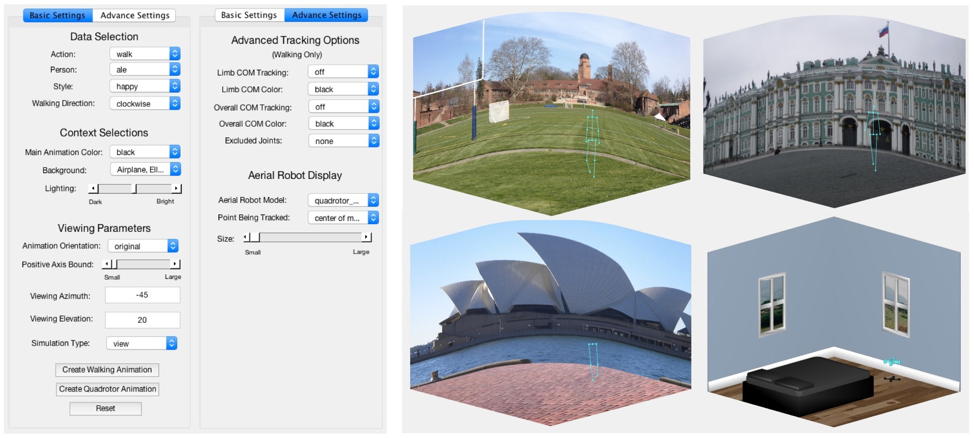
\includegraphics[width=.95\columnwidth]{madi3.png}
\caption{This figure contains a screen capture of one of the MATLAB Tools developed in the RAD Lab (left) to test the effect of context -- as approximated by background image and shown in created stimuli (right) -- on motion meaning.  The animation screen captures at right include a human walking at Cranbrook’s Upper Fields in Bloomfield Hills, MI (top left), a human without knees and elbows walking at the Winter Palace in St. Petersburg, Russia (top right), the lower body of a human walking at the Sydney Opera House in Australia (bottom left), and an aerial robot traversing across a virtual bedroom (bottom right).}
\label{madi2}
\end{figure}

%\begin{wrapfigure}{r}{.5\textwidth}
%\centering
%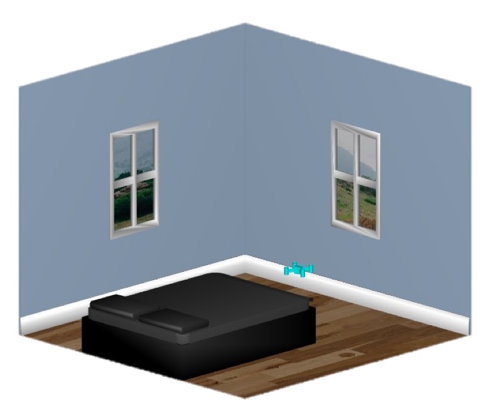
\includegraphics[width=.48\textwidth]{madi2}
%\vspace{-.1in}
%\caption{The 3D environment displayed in this screen capture of an aerial robot trajectory simulation is a bedroom.\textcolor{red}{This figure needs to demonstrate the maleability of the background and the moving figure as an experimental testbed.}}
%\label{madi2}
%\vspace{.1in}
%\end{wrapfigure}

The user studies documented in this section are a preliminary step towards understanding the relationship between movement, context, and affect recognition. The RAD Lab is also currently developing MATLAB tools that can be used to quickly and efficiently create and test stylized trajectories in various environmental contexts using data-driven approaches. Currently, the data that is being used to create the trajectories is stylized walking data obtained from an online database at the University of Glasgow \cite{ma2006motion}. However, in the future, the tools could be used as platforms for simulating choreographed movements in applicable HRI settings to quickly gauge if the movement profiles are received well and are adequate for a desired application. A screen capture of one of the current simulations is shown in Figure \ref{madi2}.


\subsection{Improving Creative Workflow for Robotic Motion Designers}

%%%%%%%%ALLI:  this paragraph might be used to enhance this section; moved from background

%Either way, experiencing this creative flow while improvising movement has underscored my desire to decrease the "compile time" when working with tools for programming robot motion. Human attention is a precious resource, easily lost, and our current interfaces are making life harder for anyone who wants to work with robots - whether that's graduate students, or artists incorporating robots into a piece, or students considering whether to study robotics.

An increasingly ubiquitous tool often used for controlling robotic systems is
the "Robot Operating System" (ROS). ROS is an open-source, Linux-based software framework which
standardizes common use-cases in robotics, such as collecting sensor data and controlling
robotic hardware. Figure \ref{alli1} shows a typical example of the interface:
programs are developed with heavy use of the command line and simulations before
code is deployed to actual robots. As a student (jokingly) put it: ``ROS is software with the sole purpose of
forcing the user to open up many windows. It also has robot applications.''
Thus, even for technical participants, the user experience with ROS is
notoriously bad. People trying to learn the software for the first time often
quit because of how frustrating and tiresome the process is.


\begin{figure}[h!]
\centering
\vspace{-.1in}
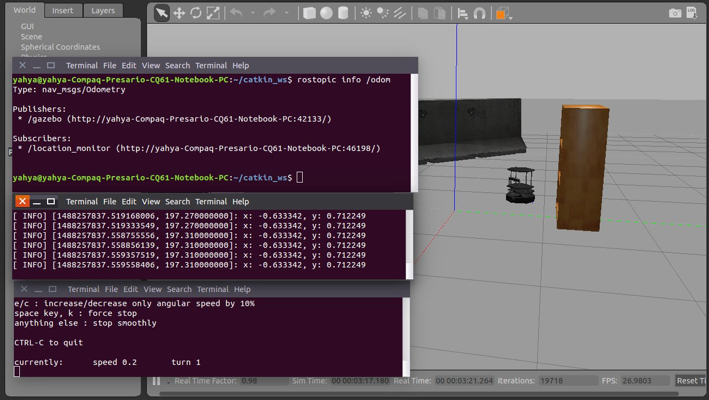
\includegraphics[width=.65\columnwidth]{alli1}
\caption{A typical ROS interface, featuring multiple command-line interfaces
and a physics-based simulator. Figure from ``An Introduction to Robot Operating
System."}
\label{alli1}
\end{figure}


When using ROS to test robot motion strategies and controllers, there are many
points in the process where the user has to stop and switch the mode of
interaction with the system. First, a text editor may be used to edit code.
Then, another window is needed to stop the currently running program, reload the
code, wait for initialization, and click to another window to view the results
on the simulator. Moreover, the user may have several different
`nodes'' running, for example, one for collecting camera data and one for controlling a robot arm. Each of these requires its own terminal window for editing and monitoring. For an example, see Figure \ref{alli1}, from an tutorial called`An
Introduction to Robot Operating System,'' aimed at absolute ROS beginners.
Several factors here are intimidating: the requirement to use the command line,
the difficulty of keeping track of all the windows, and the constant mode
switching between writing code and manually managing the programs.

Working with choreographers and dance artists drives home the need to streamline
this software. Artists are used to creative processes where the ``time to compile'' can be nearly
instant. Computer-dependent workflows, on the other hand, are often hampered by
unfriendly interfaces and long compile times.
Software limitation influence how people design projects, and
thus limit scientific exploration. One reason for this is that developers of software for robotics are often
people who do not have a clear picture of the skills and needs of
non-super-users. 
%Of course, they do an immense amount of helpful work on the
%software: thanks to the developers, we do not have to write our own network
%protocols, or hardware calibration routines. Open source software is a continual
%work-in-progress.

Interdisciplinary collaboration helps solve this problem by pulling us out of our bubble of
experience. After technical education, skills such as writing wrapper
scripts, parsing and generating low-level code, and reading through pages of
program output to debug errors, become second nature. Collaborating with people
from different backgrounds challenges assumptions about what is normal, and
highlights areas where creative workflow can be improved.
%\begin{wrapfigure}{r}{.5\textwidth}
%\centering
%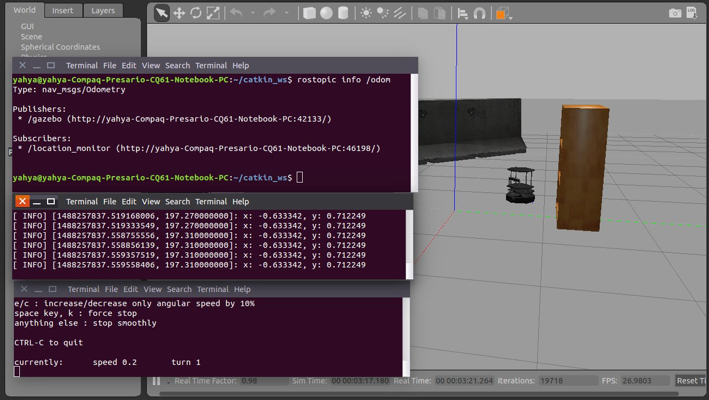
\includegraphics[width=.48\textwidth]{alli1}
%\vspace{-.1in}
%\caption{Magnetic flux density distribution of a five-segment cellular actuator when top coils in cell A B and C are excited while bottom coils are excited for cell D. Unlike serial-chains of conventional motors, the proposed distributed actuator shares the magnetic flux path resulting in better utilization of flux carrying material.}
%\label{alli1}
%\vspace{.1in}
%\end{wrapfigure}


To reduce these barriers, for technical and nontechnical alike, a project that
aims to create a live-coding interface for ROS was initiated. Live-coding is a
performing art especially prevalent in computer music, where many programming
languages and interfaces exist for creating improvised music using sound samples
and a computer. Similarly, this project is creating a domain-specific language
(DSL) which is immediately compiled to a process which publishes ROS messages to
a robot or simulator. Thus, as the user edits code, they immediately see changes
on the robot with one press of a key on their keyboard. Apart from minimizing human suffering, why
decrease barriers to learning, and decrease compile time while working? The goal
is flow: the mental state of complete absorption in an activity. When engaged in
some creative process -- coding, dancing, writing, anything -- the best work is
done when the creator is focused, feels agency over the tools they are using,
gets so wrapped up the creation that they lose track of time. If we draw an
analogy: the human as choreographer, robot as dancer, imagine how difficult it
would be to work with a dancer who randomly freezes, refuses to listen to
commands, who only speaks one specialized language that takes weeks of dedicated
practice to learn. Obviously, any human endeavor involving robots would be much
more productive if the creative process was able to flow more smoothly.

This project can be a jumping off point for formalizing other identified
choreographic ``technologies.'' These technologies are tools that
choreographers use to analyze and create movement sequences. These include
notation, motif, and video recording, as well as creative tools such as
arrangement of movements in space and time. Movements can be reversed,
retrograded, or reflected across different axes. Similar movements can be
performed at different extents or levels, or at different tempos, or with
sharper or more gradual speed changes. Moreover, dancers and choreographers have
identified heuristics that explain how these different technologies tend to
affect how audiences interpret dances: why we tend to see some dances as
frantic, others as peaceful, and what techniques create tension or capture
attention. By automating these heuristics, it may someday be possible to program
a robot at a much higher level than is currently done: the instructions from the
human to the robot will be more similar to those of a choreographer. We are far
from this point today, but by collaborating with artists and movement
observation experts, we can accelerate progress toward this goal.

\subsection{Embodied Practice in Teleoperation}

The movement activities prove an easy, almost rapid-prototyping, ground for envisioning the kinespheres for different robotic platforms without having to go through extensive testing or simulation. Developing a plan for labeling different poses without having to do a trial-and-error method in code saves a significant amount of time.  When working with a two-armed platform, exercises like Laban's movement scales help researchers mirror the platform with their own body. Even when the challenge arose to label a one-armed platform, the extensive study of how our own bodies might adapt to a similar challenge saved time in formulating motion control algorithms for such a platform.
	
This is the case when developing platform-invariant spatial commands for the robots. Traditionally, for defining a task-oriented movement for a robot, it requires information about the individual parts of the robot, the way these parts are connected in the robot, their physical properties and the mathematical model behind them. After that, based on the task at hand, different path planning techniques can be used to execute the movement. 

Key inspiration for platform-invariance in spatial commands for robots comes from LBMS. The relationship between Body and Space in LBMS provides terminologies for movements that can be applied to different human morphologies irrespective of the differences in physical features and forms (indeed, all humans have at least slightly different morphologies). 

In this work, we had to undergo similar simplification in our design. While the original idea of Body-Space contains a lot of details about its components, for example, it allows different kinesphere shapes for different possible movements, and it allows a continuous range of kinesphere sizes, we had to simplify the details to be able to implement them in a practical way.  

\begin{figure}[h!]
\centering
\vspace{-.1in}
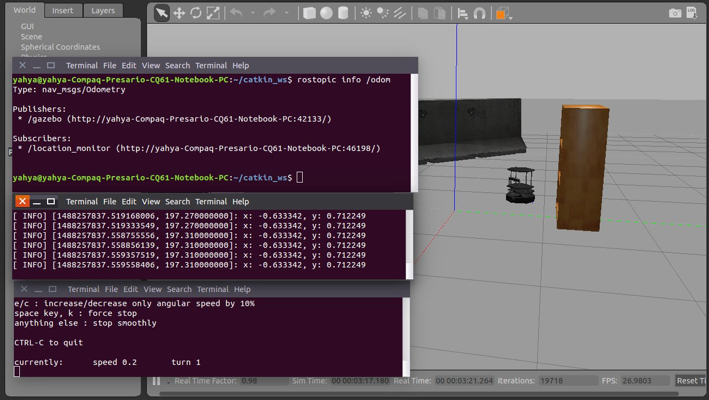
\includegraphics[width=.65\columnwidth]{alli1}
\caption{\textcolor{red}{need a single figure that shows embodied relationship to framework; cite RAS article}}
\label{alli1}
\end{figure}

In our implementation, we have restricted the implementation to the robots with serial link chains (or roughly speaking, arms).  We have fixed the kinesphere shape to a sphere, restricted the number of spatial directions because the robot we are working with doesn’t have as much dexterity as humans. Furthermore, we have restricted the kinesphere to only three kinesphere sizes, which means this framework can allow the movement up to three predefined distances. These restrictions have been made to allow for the ease of implementation.  Starting explicitly in an embodied place helps to bring these approximations to the forefront; \textcolor{red}{top-down}.


\subsection{Movement Strategies in Locomotion}
\textcolor{red}{condense; fix POV}

One of the first projects I consulted on was about re-designing the robot gait (insert all the proper terminology – title of project etc. here) Amy and Umer were interested in seeing if they could design a weight shift/locomotion system that would allow a robot to move from the “pelvic core” vs. through actuators on the ankles. We wanted to explore the many mappings of the Body and Space to see what we could determine about our movement patterns and how to “translate” or “create” a similar pattern in a robot. This desire to more accurately replicate human locomotor patterns is not only about expressivity, but it is in fact also about efficiency. 

I entered this work with them through the Body Component of LBMS and specifically through the practice of Bartenieff Fundamentals, a set of principles and movement sequences that seeks to optimize the supportive relationship between body organization and movement intention. I wanted Umer to learn about his own body patterns and experience his own weight shift from the pelvic core, experiencing dynamic alignment and optimizing his own efficiency in locomotion. We spent some sessions changing our relationship to gravity by working on the floor, locomoting through the space, studying skeletal anatomy and working through an experiential anatomy approach. In this work Umer gained insight into his own movement capacity and was then able to use that embodied experience to guide and inform his engineering of a “core actuated’ robot. I supported the development of the work and continued to answer questions, consult on ideas and move with the engineers.

Our lab works in the broader area of robot motion planning and control problems. For a typical problem at hand, we have to understand the low level details about a robot’s movement, including the behavior of individual actuators among others, before defining a complex motion profile for the whole body. For example, in making a legged robot walk some distance, a mathematical model for the individual joints and links is needed, and then a motion profile has to be derived for these individual elements to give a whole body movement that satisfies walking.


\begin{figure}[h!]
\centering
\vspace{-.1in}
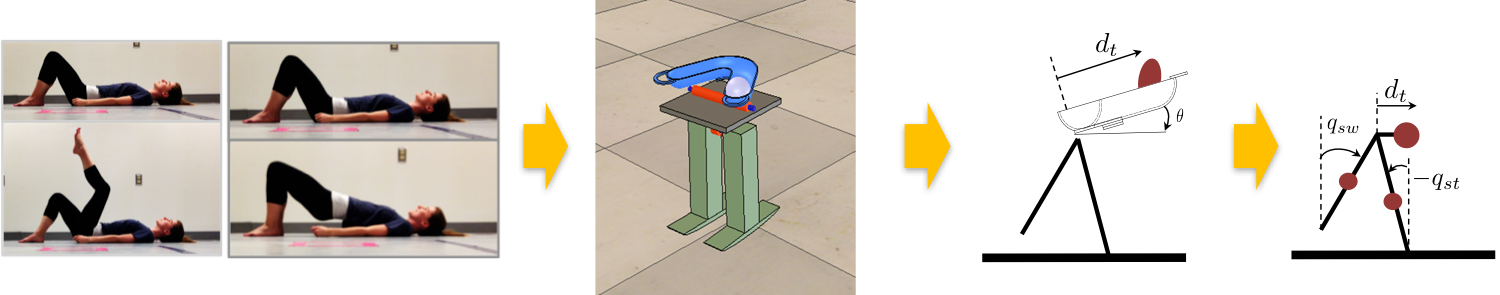
\includegraphics[width=.98\columnwidth]{walker}
\caption{Top-down design process: from embodied exercises practice by researchers (left) to a proposed bipedal robotic platform design (middle) to a simplified model, with only three degrees of freedom, for mathematical modeling (right).  \textcolor{red}{cite papers}}
\label{walker}
\end{figure}

On the other hand, in arts and more specifically, dance, description of a movement, does not involve as much technical detail as in the above example because traditionally these descriptions are meant for humans which are extremely articulate in understanding high-level motion commands and performing them. In the Embodied Movement Analysis, the field our lab works in collaboration with, is similar in this sense as its literature contains basic high-level principles about movement in humans without explicating details about the individual movement element inside the human body. 

This can be explained with the help of a project going on in our lab that is on developing a biped robot with core-located actuation. This project is inspired from abstract high-level ideas mentioned regarding human walking in the embodied movement analysis literature. As mentioned in [1], human walking is composed of three high-level movements: Thigh Lift, Forward Pelvic Shift and Lateral Pelvic Shift (word ‘core’ is also used interchangeably with pelvis). Even though these overarching ideas may be missing the low-level essential details in the execution phase, one has to go through the standard somatic exercises to get a full grasp of these ideas. That is why, our design team went through a training session with a Certified Movement Analyst (CMA) to fully grasp the idea of these movements. This included, lying down on the floor in a movement studio, identifying our cores, and realizing its related movements in walking.


As mentioned earlier, one of the projects we are working on, is the design of a bipedal walker with core-located actuation. This is inspired from the concept of a highly articulate Core in humans, which can be considered a mobile, actuated mass on top of legs in a bipedal robot. It is expected that with such a structure it may be possible to introduce a variety of gaits in a bipedal robot. 

To initiate the design process, we went through a training session with a CMA who explained to us in a traditional embodied fashion, the main principles of walking. After that, the design team spent a few brainstorming sessions and design iterations to come up with a conceptual core design (as shown in Fig. 1). 

This design consists of a tray structure that has a channel for a heavy ball of mass to roll over it. The idea of using this tray is to allow the ball to move both in the sagittal and the lateral direction just like humans shift their own centers of mass in the sagittal and lateral directions. This tray design has a U-shape with length and width of this ‘U’ being the design variables. This tray structure sits on top of the two legs in the robot (as shown in the Fig. 2). Using the idea of a rolling ball to move the center of mass, and the legs moving to locomote the robot, we were able to produce a walking motion [4].

Using this model, it is possible to mimic the movements of core in humans in both sagittal and lateral manner. By changing the length ‘l’ and width ‘w’ of the tray, we can decide how much the ball can move in sagittal and lateral direction, respectively, and as a result, the movement of robot in the respective directions can be controlled too.

For planning a movement on the robot, the design question is simplified to divide the main objective into a handful of goals that are achievable with the available technology. This simplification is accompanied with a set of suitable assumptions that create a specific scenario, and ultimately a rather simplified version of the original movement is realized. Then afterwards, the assumptions are gradually relaxed to allow more complicated versions of this simpler movement. 

Relating it to the biped robot project, we could not have started right away with designing a core structure that was as articulate as it is in humans. As we started, we did not know what control and actuation policies could result in a human-like behavior for that. Therefore, we started off with simplifying the core to a reduced degree of freedom system. 

After we came up with the initial design for the biped as shown in the Fig. 2, we went through two more design iterations for simplification. At first, we simplified the tray structure to a planar version where the ball was only allowed to roll along the length of the tray, while the tray could still do the pitching movement. In the second iteration, however, we restricted the tray pitch angle such that the ball then could move only in the sagittal direction. With this simplified design, it was much easier to model how the legs and the ‘core’ behaved with respect to each other. Therefore, we designed control strategies for this structure and showed that walking could be achieved ([5]). These iterations are graphically illustrated in the Fig. 3. In the next iterations, we will gradually remove the restrictive assumptions to ultimately design walking for a three dimensional bipedal robot.



\subsection{Animate Meaningful Artificial Characters}

\textcolor{red}{Ishaan, Reika, and Alexandra; cite pending HRI paper; observations of birds, pooh, etc (I and A); relationship to embodied practice (R); implementation in character minus kansei (I); provide a single image -- maybe just of someone watching a character and taking handwritten notes}

\subsection{Design of Impact on Subjective Experience (Through an Interactive Installation for Outreach)}

\textcolor{red}{Ishaan and Nov and Catie and Amy}

\textcolor{red}{Given that context is SO important for movement interpretation and creating meaninful characters, this project attempts to manipulate that context through priming experiences that change participants' subjective experience of an artificial agent.}

Through an artistic collaboration in the form of a one month residency with choregrapher Catie Cuan, an interactive performance was created.  The first week’s practice largely included understanding the technology in the lab and how it relates to its users.  Why does a NAO have a default “voice” that sounds like a child’s?  How does one power up the Baxter robot and input movement sequences?  The second and third weeks involved a series of experiments with the robots, from hugging a Baxter to synchronizing the quadcopters to music.  A narrative began to emerge from these experiments.  The translation of movement from a human to a machine and vice versa was both fascinating and frustrating.  An arm circle articulated by a human becomes an oversimplified imitation when “translated” to a robot with two arms.  The fourth week organized the existing experiments, both Catie/robot and audience participant/robot experiments, into a showing for the public.  It was a performance largely witnessed by members of the UIUC engineering community, an arguably atypical group for a dance performance.  

The work in progress resulted in a few key themes to continue exploring.  1) The Hidden Human Network Many technologies are powered by humans for the benefit of each other, but often this network is occluded, leaving a machine seeming quite intelligent, e.g., IBM’s Watson, which is powered by the webpage postings of users all over the Internet.  2) Are humans becoming more robot-like? This question was originally posed in the reverse, but upon further inspection, it is easy to argue that the rich adaptability of humans is heavily exploited in emerging technologies (more than any particularly successful imitation of biology).  With these changes, are humans finding social structures like family or friendships in embodied and personal technology experiences?  3) Time to Compile How long does it take to find resolution with or understanding of different technologies?  How long before we iterate on the first design and find a second?  Who gets to investigate the inner-workings of these machines before?  When have we assimilated a new technology permanently? How will we change?

\section{Discussion: Establishing Principles for Interdisciplinary Study Between Robotics and Dance}

\textcolor{red}{Amy's responsibility; she will cannibalize some other sections to get started}

Make explicit connections between all

\begin{itemize}
\item Value systems (rhetorical vs phenomenological; papers vs other output)
\item Iteration time (quite distinct between disciplines)
\item Body-based exploration
\item Articulating, describing, and observing movement (as a valued activity)
\item Using context to inform character development (meaningless without)
\end{itemize}

\subsection{Framing of Activity, Values, and Norms}

\subsection{Irreplaceable Body-Based Learning in Robotics}

\textcolor{red}{can pull (or repeat) several blocks from elsewhere where students are citing how experiences helped}

\subsection{Objective, Qualitative Movement Observation (to Support Subjective Conclusions)}

\textcolor{red}{merge last two bullets; subjective quantification?}
\textcolor{red}{style vs affect}

\subsection{Logistics of Working with Dancers, Choreographers, and CMAs}

\textcolor{red}{guidelines, and justification of, for publishing}  Examples of work leveraging CMA expertise that is not acknowledged with co-authorship \cite{salaris2017robot}; this needs to be framed as a problem both for attribution and for necessarily subjective interpretations made by CMAs.  \textcolor{red}{pull quotes from review}

%This section may be divided by subheadings. It should provide a concise and precise description of the experimental results, their interpretation as well as the experimental conclusions that can be drawn.

%%%%%%%%%%%%%%%%%%%%%%%%%%%%%%%%%%%%%%%%%%
%\subsection{Subsection}
%
%\subsubsection{Subsubsection}
%
%Bulleted lists look like this:
%\begin{itemize}[leftmargin=*,labelsep=5.8mm]
%\item	First bullet
%\item	Second bullet
%\item	Third bullet
%\end{itemize}
%
%Numbered lists can be added as follows:
%\begin{enumerate}[leftmargin=*,labelsep=4.9mm]
%\item	First item 
%\item	Second item
%\item	Third item
%\end{enumerate}
%
%The text continues here.
%
%\subsection{Figures, Tables and Schemes}
%
%All figures and tables should be cited in the main text as Figure 1, Table 1, etc.
%
%\begin{figure}[H]
%\centering
%
\includegraphics[width=3 cm]{logo-mdpi}
%\caption{This is a figure, Schemes follow the same formatting. If there are multiple panels, they should be listed as: (\textbf{a}) Description of what is contained in the first panel. (\textbf{b}) Description of what is contained in the second panel. Figures should be placed in the main text near to the first time they are cited. A caption on a single line should be centered.}
%\end{figure}   
%
%\begin{table}[H]
%\caption{This is a table caption. Tables should be placed in the main text near to the first time they are cited.}
%\centering
%%% \tablesize{} %% You can specify the fontsize here, e.g.  \tablesize{\footnotesize}. If commented out \small will be used.
%\begin{tabular}{ccc}
%\toprule
%\textbf{Title 1}	& \textbf{Title 2}	& \textbf{Title 3}\\
%\midrule
%entry 1		& data			& data\\
%entry 2		& data			& data\\
%\bottomrule
%\end{tabular}
%\end{table}
%
%\subsection{Formatting of Mathematical Components}
%
%This is an example of an equation:
%
%\begin{equation}
%\mathbb{S}
%\end{equation}
%
%%% If the documentclass option "submit" is chosen, please insert a blank line before and after any math environment (equation and eqnarray environments). This ensures correct linenumbering. The blank line should be removed when the documentclass option is changed to "accept" because the text following an equation should not be a new paragraph. 
%Please punctuate equations as regular text. Theorem-type environments (including propositions, lemmas, corollaries etc.) can be formatted as follows:
%%% Example of a theorem:
%\begin{Theorem}
%Example text of a theorem.
%\end{Theorem}
%
%The text continues here. Proofs must be formatted as follows:
%
%%% Example of a proof:
%\begin{proof}[Proof of Theorem 1]
%Text of the proof. Note that the phrase `of Theorem 1' is optional if it is clear which theorem is being referred to.
%\end{proof}
%The text continues here.

%%%%%%%%%%%%%%%%%%%%%%%%%%%%%%%%%%%%%%%%%%
%\section{Discussion}
%
%Authors should discuss the results and how they can be interpreted in perspective of previous studies and of the working hypotheses. The findings and their implications should be discussed in the broadest context possible. Future research directions may also be highlighted.

%%%%%%%%%%%%%%%%%%%%%%%%%%%%%%%%%%%%%%%%%%
%\section{Materials and Methods}
%
%Materials and Methods should be described with sufficient details to allow others to replicate and build on published results. Please note that publication of your manuscript implicates that you must make all materials, data, computer code, and protocols associated with the publication available to readers. Please disclose at the submission stage any restrictions on the availability of materials or information. New methods and protocols should be described in detail while well-established methods can be briefly described and appropriately cited.
%
%Research manuscripts reporting large datasets that are deposited in a publicly available database should specify where the data have been deposited and provide the relevant accession numbers. If the accession numbers have not yet been obtained at the time of submission, please state that they will be provided during review. They must be provided prior to publication.
%
%Interventionary studies involving animals or humans, and other studies require ethical approval must list the authority that provided approval and the corresponding ethical approval code. 

%%%%%%%%%%%%%%%%%%%%%%%%%%%%%%%%%%%%%%%%%%
\section{Conclusions: Toward Widespread Collaboration Between Dancers and Roboticists}
\begin{center}
\textit{...the truest creativity of the digital age came from those who connected the arts and sciences.}
\end{center}
\begin{flushright}
%\vspace{-.2in}
-- The Innovators \cite{isaacson2014innovators}
\end{flushright}

This section is not mandatory, but can be added to the manuscript if the discussion is unusually long or complex. \textcolor{red}{Amy will write at end to summarize main points (once they congeal).}

%%%%%%%%%%%%%%%%%%%%%%%%%%%%%%%%%%%%%%%%%%
\vspace{6pt} 

%%%%%%%%%%%%%%%%%%%%%%%%%%%%%%%%%%%%%%%%%%
%% optional
%\supplementary{The following are available online at www.mdpi.com/link, Figure S1: title, Table S1: title, Video S1: title.}

%%%%%%%%%%%%%%%%%%%%%%%%%%%%%%%%%%%%%%%%%%
\acknowledgments{All sources of funding of the study \textcolor{red}{name all in lab} should be disclosed. Please clearly indicate grants that you have received in support of your research work. Clearly state if you received funds for covering the costs to publish in open access.}

%%%%%%%%%%%%%%%%%%%%%%%%%%%%%%%%%%%%%%%%%%
\authorcontributions{For research articles with several authors, a short paragraph specifying their individual contributions must be provided. The following statements should be used ``X.X. and Y.Y. conceived and designed the experiments; X.X. performed the experiments; X.X. and Y.Y. analyzed the data; W.W. contributed reagents/materials/analysis tools; Y.Y. wrote the paper.'' Authorship must be limited to those who have contributed substantially to the work reported.}

%%%%%%%%%%%%%%%%%%%%%%%%%%%%%%%%%%%%%%%%%%
\conflictsofinterest{The authors declare no conflict of interest.  The founding sponsors had no role in the design of the study; in the collection, analyses, or interpretation of data; in the writing of the manuscript, and in the decision to publish the results.} 

%%%%%%%%%%%%%%%%%%%%%%%%%%%%%%%%%%%%%%%%%%
%% optional
\abbreviations{The following abbreviations are used in this manuscript:\\

\noindent 
\begin{tabular}{@{}ll}
MDPI & Multidisciplinary Digital Publishing Institute\\
DOAJ & Directory of open access journals\\
LBMS & Laban/Bartenieff Movement Studies
\end{tabular}}

%%%%%%%%%%%%%%%%%%%%%%%%%%%%%%%%%%%%%%%%%%
%% optional
\appendixtitles{no} %Leave argument "no" if all appendix headings stay EMPTY (then no dot is printed after "Appendix A"). If the appendix sections contain a heading then change the argument to "yes".
%\appendixsections{multiple} %Leave argument "multiple" if there are multiple sections. Then a counter is printed ("Appendix A"). If there is only one appendix section then change the argument to "one" and no counter is printed ("Appendix").
%\appendix
%\section{}
%\subsection{}
%The appendix is an optional section that can contain details and data supplemental to the main text. For example, explanations of experimental details that would disrupt the flow of the main text, but nonetheless remain crucial to understanding and reproducing the research shown; figures of replicates for experiments of which representative data is shown in the main text can be added here if brief, or as Supplementary data. Mathematical proofs of results not central to the paper can be added as an appendix.
%
%\section{}
%All appendix sections must be cited in the main text. In the appendixes, Figures, Tables, etc. should be labeled starting with `A', e.g., Figure A1, Figure A2, etc. 

%%%%%%%%%%%%%%%%%%%%%%%%%%%%%%%%%%%%%%%%%%
% Citations and References in Supplementary files are permitted provided that they also appear in the reference list here. 

%=====================================
% References, variant A: internal bibliography
%=====================================
%\reftitle{References}
%\begin{thebibliography}{999}
%% Reference 1
%\bibitem[Author1(year)]{ref-journal}
%Author1, T. The title of the cited article. {\em Journal Abbreviation} {\bf 2008}, {\em 10}, 142-149, DOI.
%% Reference 2
%\bibitem[Author2(year)]{ref-book}
%Author2, L. The title of the cited contribution. In {\em The Book Title}; Editor1, F., Editor2, A., Eds.; Publishing House: City, Country, 2007; pp. 32-58, ISBN.
%\end{thebibliography}

% The following MDPI journals use author-date citation: Arts, Econometrics, Economies, Genealogy, Humanities, IJFS, JRFM, Laws, Religions, Risks, Social Sciences. For those journals, please follow the formatting guidelines on http://www.mdpi.com/authors/references
% To cite two works by the same author: \citeauthor{ref-journal-1a} (\citeyear{ref-journal-1a}, \citeyear{ref-journal-1b}). This produces: Whittaker (1967, 1975)
% To cite two works by the same author with specific pages: \citeauthor{ref-journal-3a} (\citeyear{ref-journal-3a}, p. 328; \citeyear{ref-journal-3b}, p.475). This produces: Wong (1999, p. 328; 2000, p. 475)

%=====================================
% References, variant B: external bibliography
%=====================================
\externalbibliography{yes}
\bibliography{papers}

%%%%%%%%%%%%%%%%%%%%%%%%%%%%%%%%%%%%%%%%%%
%% optional
%\sampleavailability{Samples of the compounds ...... are available from the authors.}

%%%%%%%%%%%%%%%%%%%%%%%%%%%%%%%%%%%%%%%%%%
\end{document}

